\section{SAT}

	\begin{frame}[plain]
		\vfill
		\centering
		\begin{beamercolorbox}[sep=8pt,center,shadow=true,rounded=true]{title}
			\textbf{\usebeamerfont{title}\insertsectionhead}\par%
			\color{polimiblue}\noindent\rule{10cm}{1pt} \\
			\textbf{The SATisfiability problem}
		\end{beamercolorbox}
		\vfill
	\end{frame}

	\subsection{Problem Definition}
		\begin{frame}{Problem Definition}
			\small
			 Let $X\equiv\{x_1, x_2, ..., x_n\}$ be a set\\
			 \vspace{0.1cm}
			 Then $x_k$ and its negations $\overline{x}_k$ are called literals and the set of all literals is denoted by $X^{'}=\{x_1, \overline{x}_1, ..., x_n, \overline{x}_n\}$\\
			 \vspace{0.1cm}
			 The set of all subsets of $X^{'}$ is denoted by $\mathcal{F}(X^{'})$ and an element $C\in\mathcal{F}(X^{'})$ is called a clause\\
			 
			 \vspace{0.3cm}
			 
			 \textbf{SAT problem:} \emph{Given a set $X=\{x_1, x_2, ..., x_n\}$ and a set of clauses $\mathcal{C}=\{C_1, C_2, ..., C_m\}$ of clauses, determine whether $\mathcal{C}$ is satisfiable or not.\\}
			 
			 \vspace{0.3cm}
			 
			 In the literature we find the problem typically identified as k-SAT where we need to consider:
			 \begin{itemize}
			 	\item[1.] The number of variables on which the problem is defined: \textbf{n}
			 	
			 	\item[2.] The number of clauses on which the problem is defined: \textbf{m}
			 	
			 	\item[3.] The maximal length of the clauses in the problem: \textbf{k}
			 \end{itemize}
		\end{frame}
	
		\begin{frame}{SAT example}
			\small
			Consider the following two clauses defining a 3-SAT problem over the variables $x_1, x_2, x_3$:
			\begin{center}
				$C_1=\{\overline{x}_1, x_2, x_3\}$
				\hspace{0.5cm}
				$C_2=\{x_1, \overline{x}_2, x_3\}$
			\end{center} 
			Corresponding to the \emph{Conjunctive Normal Form}:
			\begin{equation*}
				\centering
				CNF=(\overline{x}_1\lor x_2\lor x_3)\land(x_1\lor\overline{x}_2\lor x_3)
			\end{equation*}
			\vspace{1cm}
			\begin{minipage}{0.38\textwidth}
				That we represented in a quantum circuit, by exploiting the relations between the quantum and classical operations, as represented in the picture on the right
				\vspace{1.2cm}
			\end{minipage}
			\hfill
			\begin{minipage}{0.6\textwidth}
				\centering
				\begin{figure}[h]
					\centering
					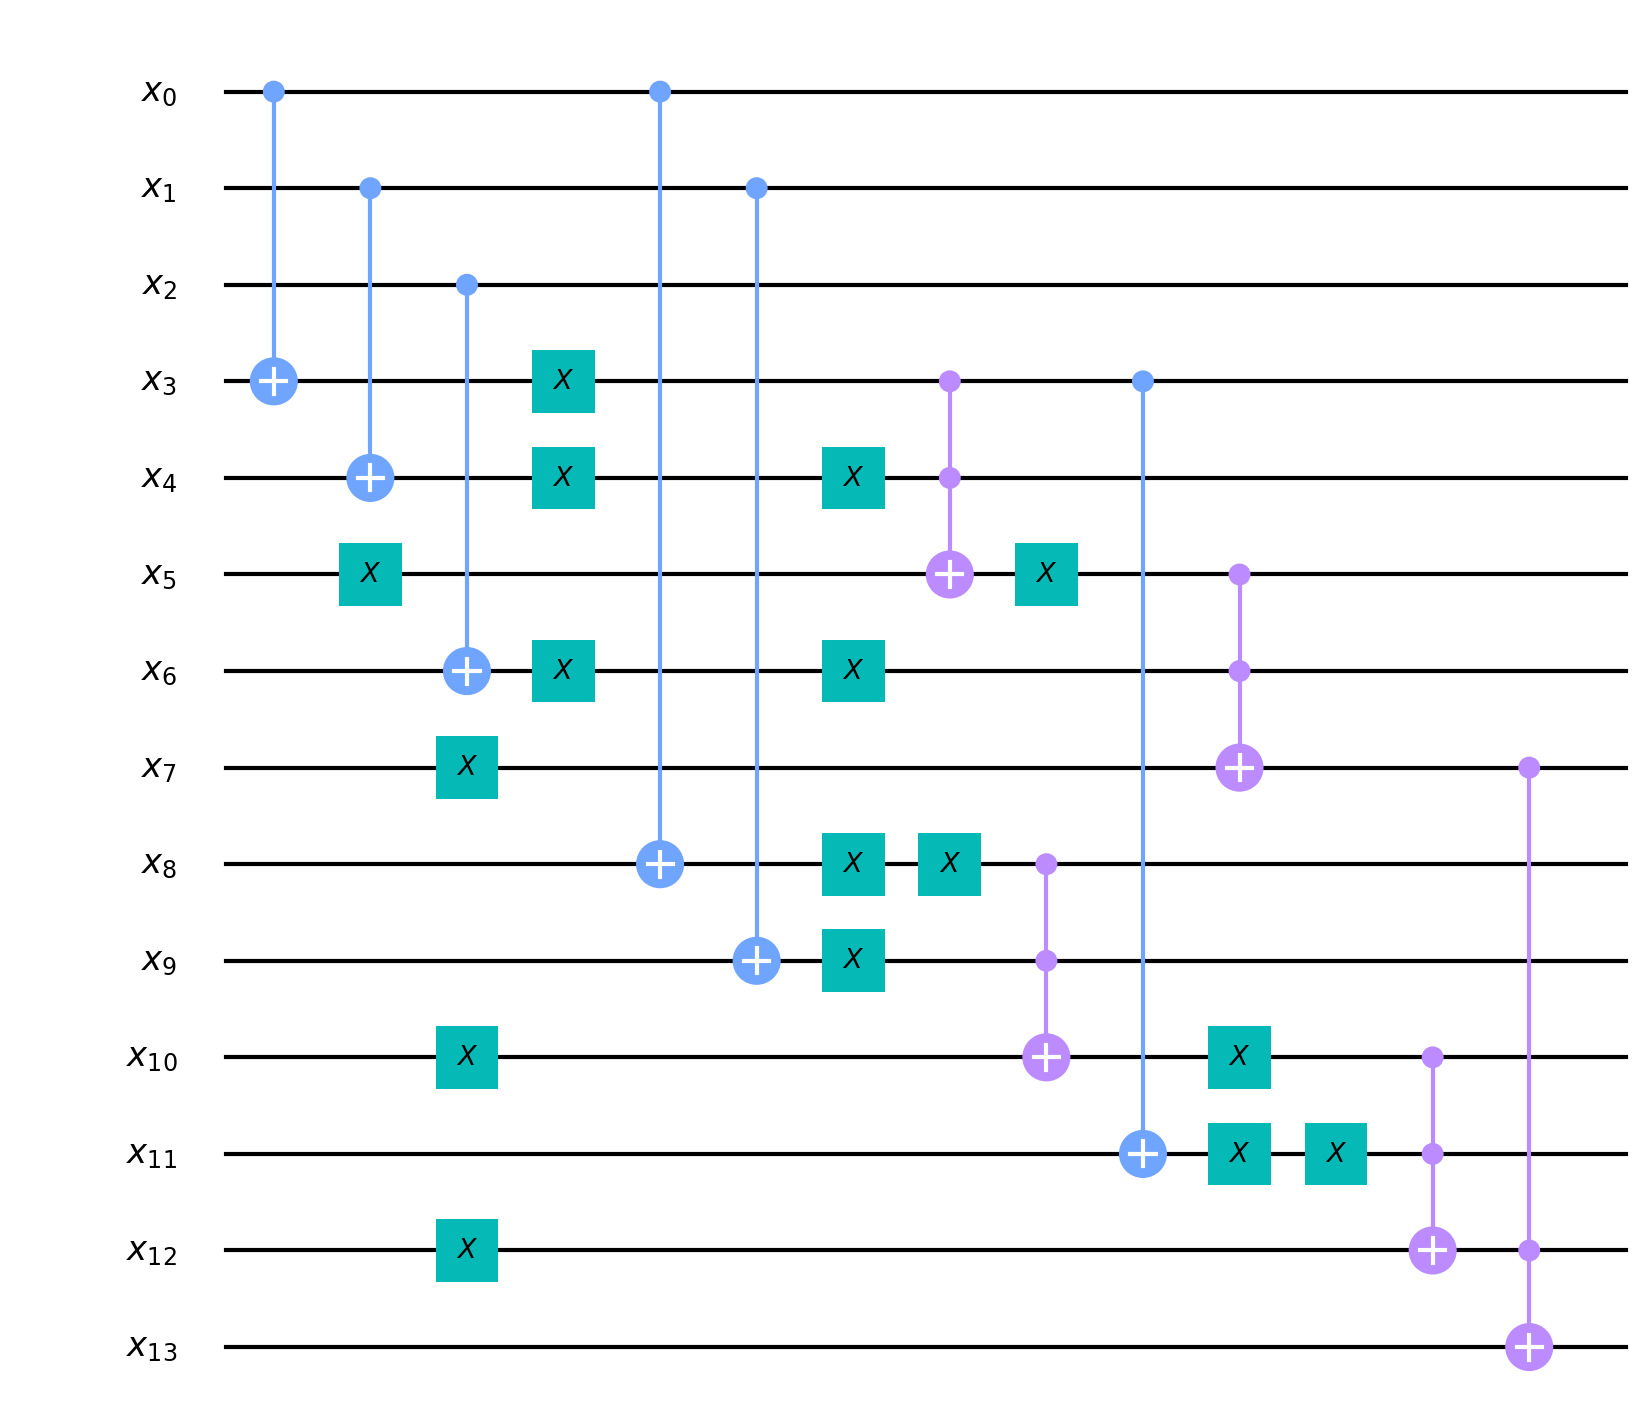
\includegraphics[scale=0.19]{exampleSAT.png}
				\end{figure}
			\end{minipage}
		\end{frame}
	
	\subsection{Classical Solver}
		\begin{frame}{Classical Solver}
			\small
			Classical solvers for the SAT problem are widely studied for their importance in applications, in particular \textbf{Artificial Intelligence} \\
			
			\vspace{0.3cm}
			
			\emph{Deterministic} and \emph{Nondeterministic} algorithms are used to solve SAT instances, with a focus in particular for the 3-SAT problem:
			\begin{itemize}
				\item[$\bullet$] <1-> [Kutzkov and Scheder, 2010] $\mathcal{O}(1.439^n)$ \textbf{[Det]}
				
				\item[$\bullet$] <2-> [Makino, Tamaki and Yamamoto, 2013] $\mathcal{O}(1.3303^n)$ \textbf{[Der]}
				
				\item[$\bullet$] <3-> [Iwama, Seto Takai and Tamaki, 2010] $\mathcal{O}(1.32113^n)$ \textbf{[Rand]}
				
				\item[$\bullet$] <4-> [Hertli, Moser and Scheder, 2010] $\mathcal{O}(1.32065^n)$ \textbf{[Rand]}
				
				\item[$\bullet$] <5-> [Hertli, 2011] $\mathcal{O}(1.30704^n)$ \textbf{[Rand]}
			\end{itemize}
			\onslide<6->{In our study we considered an efficient classical search algorithm based on backtracking, able to solve the general \textbf{k-SAT} algorithm}
		\end{frame}
	
	\subsection{Quantum Solver}
		\begin{frame}{Quantum Solver}
			To face the problem of solving the SAT in the quantum world we realized \textbf{3} implementations:
			\begin{itemize} % todo choose se usare il notebook o direttamente da git
				\item[1.] \textbf{Qiskit's general solver} (\href{https://github.com/Askarpour/sw2_quantum_research/blob/master/Piro/Code/Quantum/quantumSat.ipynb}{Jupyter Notebook})
				
				\item[2.] \textbf{Decision Version}
				
				\item[3.] \textbf{Generalized exactly-1 k-SAT solver}
			\end{itemize}
			We now focus on describing how the general solver for the \textbf{Exactly-1 k-SAT} problem works, considering an example to go through the 3 steps of \textbf{Grover's algorithm}\\
			
			\vspace{0.3cm}
			
			Then a short \textbf{demo} on how to run the solver on the same example will prove the consistency of what has been described
		\end{frame}
	
		\begin{frame}{Exactly-1 k-SAT solver}
			\small
			\textbf{Definition:} \emph{Given a k-SAT problem we want to determine a satisfying assignment containing one true literal per clause.\\}
			
			\vspace{0.3cm}
			
			We realized the generalized version provided in [Nannicini, 2020] now able to solve the \textbf{exactly-1 k-SAT} problem with an arbitrary number of variables, clauses and in particular k \\
			
			\vspace{0.6cm}
			
			\begin{minipage}{0.5\textwidth}
				We implemented the solver using \textbf{Grover's search} algorithm to find the satisfiable solution. We now show how the three steps are generalized for the case of a 4-SAT problem over $n=4$ variables and $m=4$ clauses
			\end{minipage}\hspace{1cm}
			~
			\begin{minipage}{0.3\textwidth}
				\textbf{Problem 4}\\
				$X=\{x_1, x_2, x_3, x_4\}$\\
				$C=\{C_1, C_2, C_3, C_4\}$\\
				Such that:\\
				$C_1 = \{x_1, \overline{x}_2, \overline{x}_3, \overline{x}_4\}$\\
				$C_2 = \{\overline{x}_1, x_2, \overline{x}_4\}$\\
				$C_3 = \{\overline{x}_1, \overline{x}_2, \overline{x}_3, x_4\}$\\
				$C_4 = \{\overline{x}_2, x_3, \overline{x}_4\}$
			\end{minipage}
		\end{frame}
	
		\begin{frame}{Initialization}
			\small
			\textbf{Grover's algorithm} applies to a function with an n-qubit input and a single qubit output\\
			
			\vspace{0.2cm}
			
			In this case we have \textbf{n=4} inputs and always a single output, where:
			\begin{itemize}
				\item[$\bullet$] \texttt{f\_in} is the input register of the encoded function $U_f$, of size 4
				
				\item[$\bullet$] \texttt{f\_out} is the output register of $U_f$, of size 1
			\end{itemize}
			\begin{minipage}{0.5\textwidth}
				The initialization of the algorithm consists of bringing the state in the \textbf{uniform superposition}. This is achieved by applying an Hadamard gate on all the 4 input qubits and an X gate followed by another Hadamard for the output.
				\vspace{0.5cm}
			\end{minipage}\hfill
			\begin{minipage}{0.5\textwidth}
				\centering
				\begin{figure}[h]
					\centering
					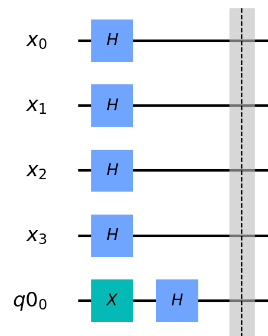
\includegraphics[scale=0.71]{initializationExample.png}
				\end{figure}
			\end{minipage}
		\end{frame}
	
		\begin{frame}{Black-box function $U_f$}
			\small
			Implementing $U_f$ is the most difficult step of the algorithm\\
			
			\vspace{0.2cm}
			
			The problem of computing $U_f$ is decomposed for each clause by introducing \textbf{m} auxiliary qubits\\
			
			\vspace{0.2cm}
			
			For each \textbf{clause} we build a circuit that bit-flips the output register of $U_f$ if and only if all the m auxiliary qubits are equal to 1\\
			
			\vspace{0.2cm}
			
			Considering the clause $C_1$ of our example we want to realize the following circuit:
			\begin{figure}[h]
				\vspace{-0.3cm}
				\centering
				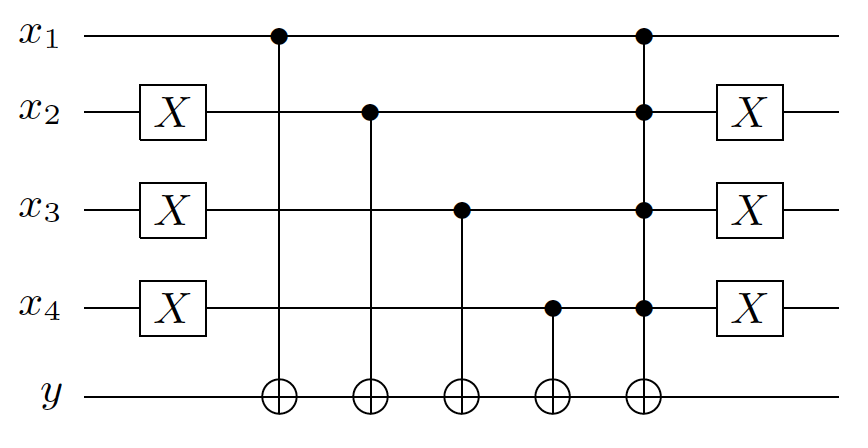
\includegraphics[scale=0.33]{theoreticalExample.png}
				\vspace{-0.3cm}
			\end{figure}
			\textbf{Unfortunately Qiskit provides only doubly-controlled NOT gates...}
		\end{frame}
	
		\begin{frame}{Qiskit solution}
			\begin{figure}
				\vspace{-1cm}
				\centering
				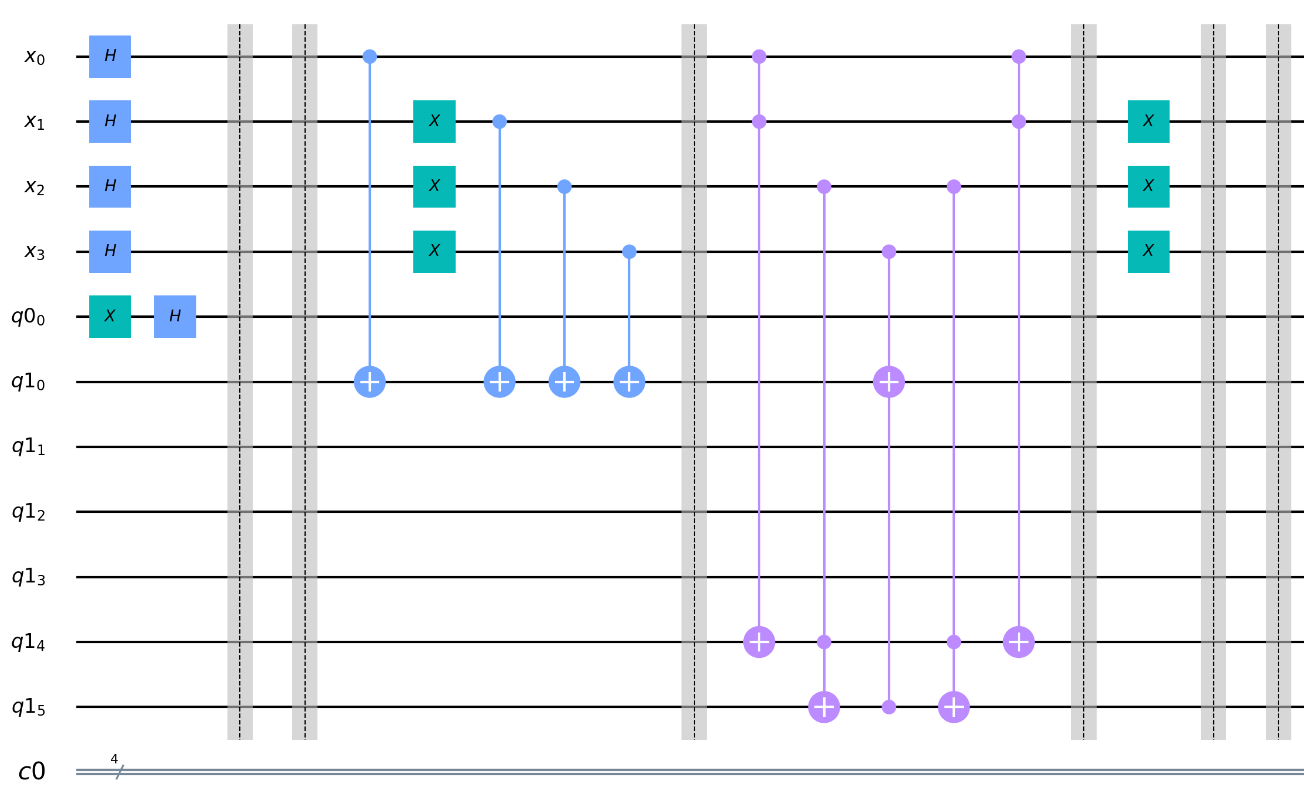
\includegraphics[scale=0.49]{ufunctionExample.png}
			\end{figure}
		\end{frame}
	
		\begin{frame}{Inversion about the average}
			The last step of \textbf{Grover's algorithm}, updating once more the coefficients of the quantum state storing the solution, can be described with a unitary matrix called $W$\\
			
			\vspace{0.2cm}
			
			The matrix $W$ is performed over the quantum state and is defined in general as:
			\begin{equation*}
				\centering
				W = (-\otimes^n\mathcal{H})D(\otimes^n\mathcal{H})
			\end{equation*}
			Also in this case we have the problem of realizing a \textbf{multiply-controlled NOT} gate, for the diagonal matrix $D$; thus a $C^{n-1}Z$ gate. In our case, with $n=4$, we will need to consider an additional ancillary qubit to implement the $C^3Z$ gate.
		\end{frame}
	
		\begin{frame}{Qiskit Solution}
			\vspace{-0.8cm}
			\centering
			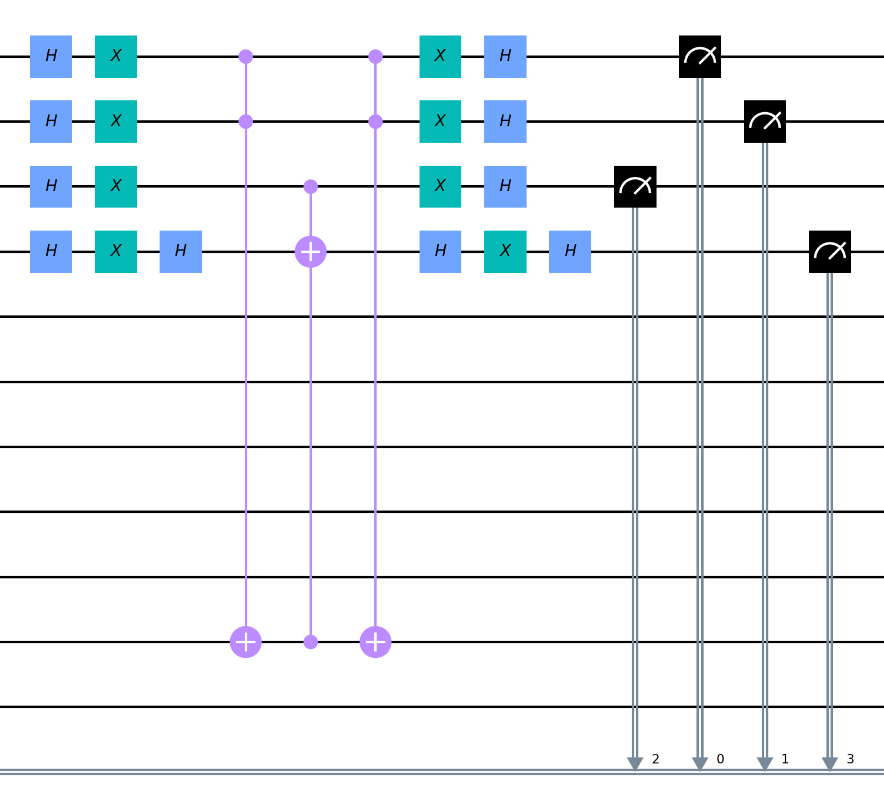
\includegraphics[scale=0.56]{averageInversionExample.png}
		\end{frame}
	
		\begin{frame}{Problem 4 Result}
			By executing the solver for the \textbf{exactly-1 Problem 4} we obtain the following solution:
			\begin{figure}[h]
				\vspace{-0.2cm}
				\centering
				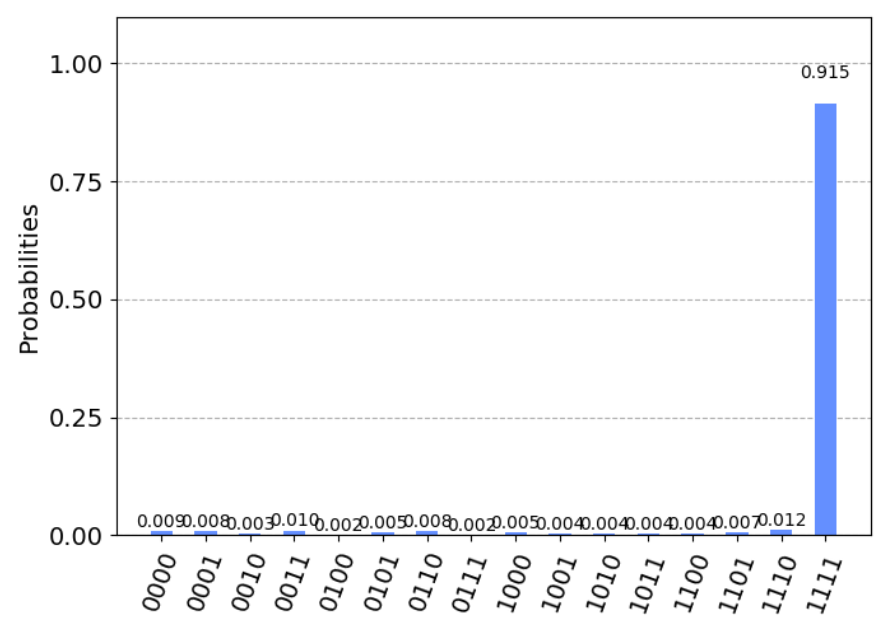
\includegraphics[scale=0.42]{resultExample.png}
				\vspace{-0.3cm}
			\end{figure}
			\textbf{Let's now do the demo to show the solver in action for the problem we considered}
		\end{frame}
	
	\subsection{Classic vs. Quantum}
		\begin{frame}{Classic vs. Quantum}
			\small
			\begin{itemize}
				\item[$\bullet$] \textbf{Complexity}
					\begin{itemize}
						\item[\tiny$\bullet$] \textbf{Space Complexity}\\
							\emph{Gates and depth explosion in Qiskit solver}\\
							\emph{Exponential growth of qubits to represent the quantum state}\\
							\emph{No-cloning principle} 
						
						\item[\tiny$\bullet$] \textbf{Time Complexity}\\
							\emph{QFT approach may lead to the number of elementary instructions}\\
							\emph{Grover's search provides a \textbf{quadratic speedup}}
					\end{itemize}
				
				\item[$\bullet$] \textbf{Implementation:} \\
					\emph{Classical and quantum algorithms do not have an exact correspondence}\\
					\emph{We have a \textbf{zoo} of quantum algorithms to be reused in order to solve our problem}\\
					\emph{The \textbf{programming paradigm} is completely changed}
			\end{itemize}
		\end{frame}
	
		\begin{frame}{Time Complexity}
			\small
			The algorithm we introduced for the classical solvers run in time
			\vspace{-0.2cm}
			\begin{equation*}
				\centering
				\mathcal{O}(T(n)poly(n))
				\vspace{-0.2cm}
			\end{equation*}
			where $T(n)$ is an exponentially growing function of n. These algorithms are based on a \textbf{polynomial-time} algorithm that outputs the satisfying assignments, if one exists, with probability at least $1/T$.\\
			
			\vspace{0.2cm}
			
			\textbf{To make a SAT problem satisfiable we will run the algorithm $\mathcal{O}(T(n))$ times}\\
			
			\vspace{0.3cm}
			
			With Grover and in particular \textbf{Amplitude Amplification} we can decide if an algorithm accepts with probability $0$ or $1/T$ running it only the $\mathcal{O}(\sqrt{T(n)})$ of the times.\\
			
			\vspace{0.2cm}
			
			In conclusion applying Grover to a k-SAT solver brings to the \textbf{quadratic speedup} we promised:
			\vspace{-0.2cm}
			\begin{equation*}
				\centering
				\mathcal{O}(\sqrt{T(n)}poly(n))
			\end{equation*}  
		\end{frame}
		
	\subsection{Conclusions}
		\begin{frame}{Conclusions}
			\begin{itemize}
				\item[1.] <1-> \textbf{Gap} between the quantum implementation and its real deploy on a device
				
				\item[2.] <2-> \textbf{Exponential growth} of the quantum state
				
				\item[3.] <3-> \textbf{Theoretical} time speedups
				
				\item[4.] <4-> \textbf{Zoo} of quantum algorithms to solve our problems
				
				\item[5.] <5-> The \textbf{role} of the computer scientist
				
				\item[6.] <6-> New \textbf{programming paradigm}
			\end{itemize}
		\end{frame}
	
		\begin{frame}{Qiskit's Contributor}
			\small
			I became contributor of the \textbf{Qiskit library} by solving the following issue
			\begin{figure}[h]
				\centering
				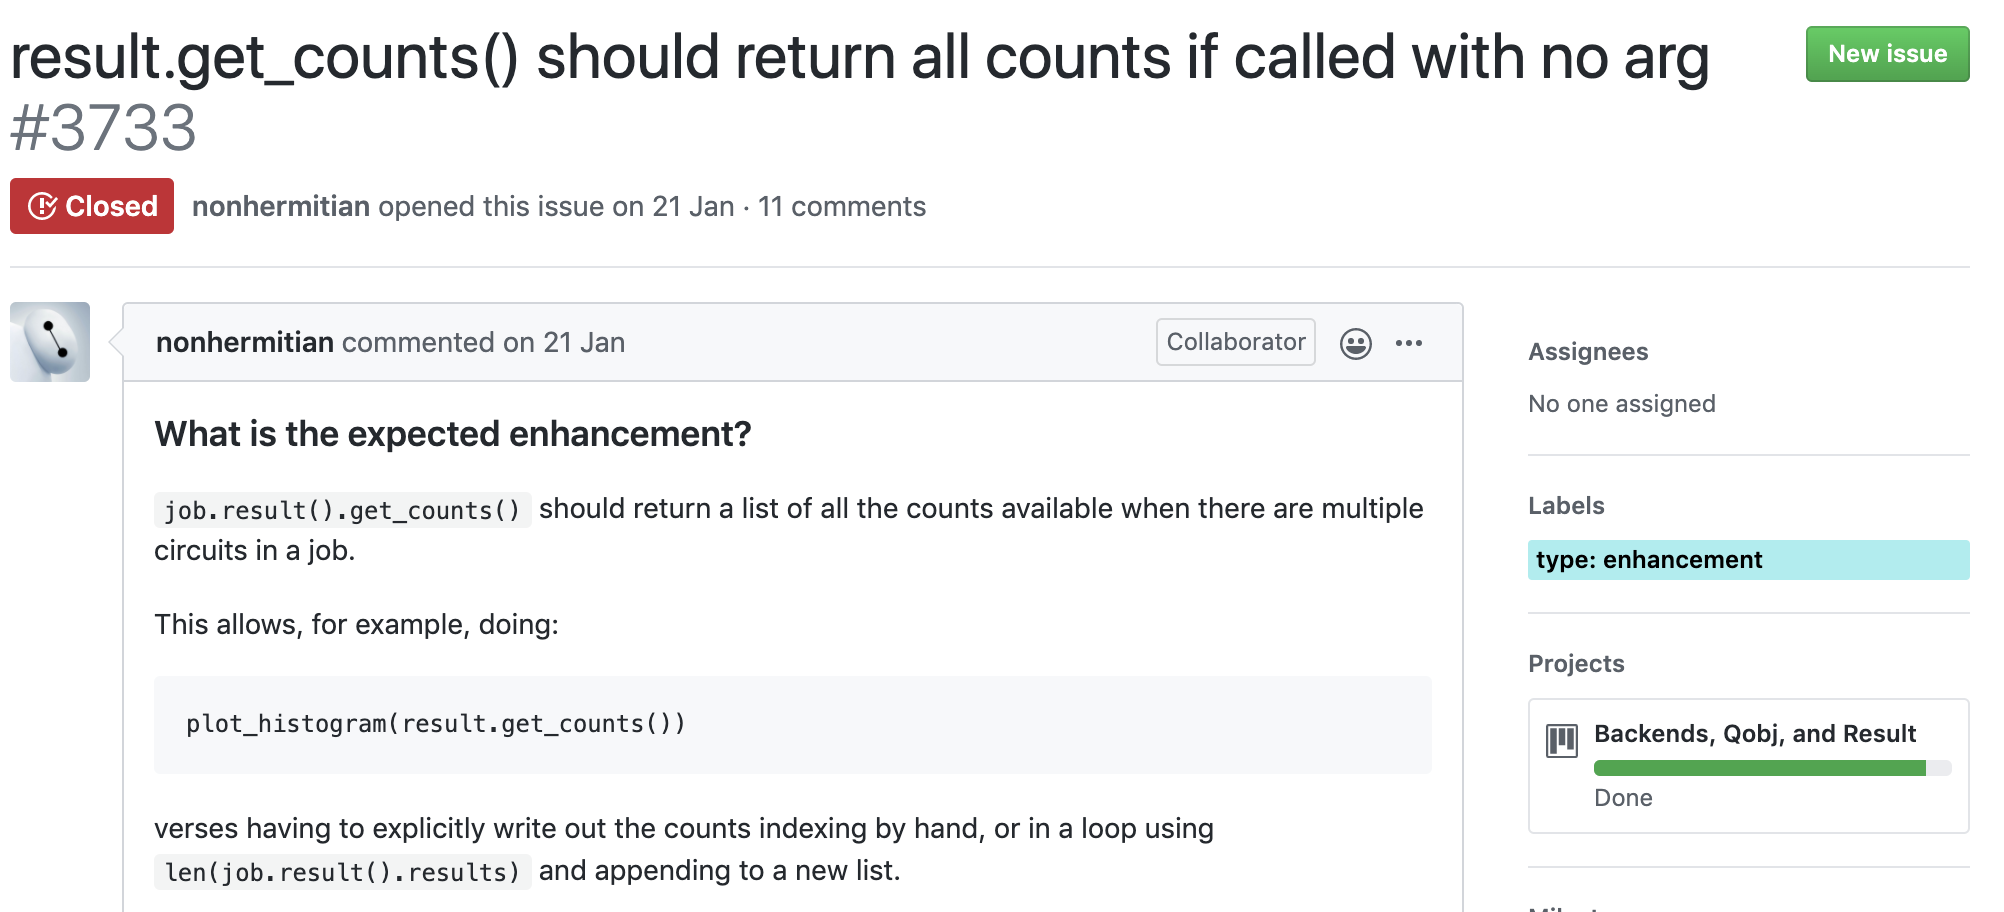
\includegraphics[scale=0.3]{qiskitIssue.png}
			\end{figure}
			Link to the \href{https://github.com/Qiskit/qiskit-terra/pull/3751}{\textbf{Pull Request}}
		\end{frame}
		